%!TEX root = ../thesis.tex
\begin{savequote}[75mm]
This is some random quote to start off the chapter.
\qauthor{Firstname lastname}
\end{savequote}

\chapter{Methods}

The Discrete Voter Model is implemented in Python 3, and the accompanying code is found in the repository noted in \hyperref[chap:appendix]{Appendix A}. A set of $6$ modules supports the Discrete Voter Model, with each implementing an aspect of the statistical framework. Those modules are:

\begin{enumerate}
  \item \texttt{phc}: creates probabilistic hypercubes
  \item \texttt{expec\_votes}: finds the expectation of votes for a candidate
  \item \texttt{prob\_votes}: finds the probability of an electoral outcome
  \item \texttt{elect}: aggregates election and electorate data
  \item \texttt{tools}: provides auxiliary functions for the model
  \item \texttt{dvm}: executes the Markov chain on a state space of hypercubes
\end{enumerate}

The modules work together to run the Discrete Voter Model on an \texttt{Election} object to generate a distribution of probabilistic hypercubes for the election. Each probabilistic hypercube encodes a probability distribution within a potential precinct of the district, and is used to extract the likely demographic voting probabilities.

These demographic voting probabilities are the goal of the ecological inference, and provide information to answer whether voting in an election is polarized by race.

\section{phc}

\newthought{The Discrete Voter Model} introduces the probabilistic hypercube (PHC) to represent the distribution of possible demographic voting probabilities in a precinct, for a candidate.

A probabilistic hypercube (PHC) is defined as a rank $n$ tensor (matrix, multidimensional array, or holor) in $\mathbb{R}^n$ space with the following characteristics:
\begin{enumerate}
  \item the component values of the cells sum to $1$
  \item each dimension corresponds to a demographic group in an electorate
  \item each cell's position, or index, represents the demographic voting probabilities of a precinct
  \item each cell's component value represents the inferred probability of that cell representing the true demographic voting probability of a precinct
\end{enumerate}

The function \texttt{make\_phc} initializes a PHC with either random or uniform cell components. The rank of the PHC corresponds to the number of demographic groups being analyzed by the model. The size of each dimension is the \textit{granularity} of the discretization, and thus the model.

For example, a PHC with granularity $100$ meant to represent $3$ demographic groups will have the shape $(100, 100, 100)$, and can be thought of as a $100 \times 100 \times 100$ matrix.

The demographic voting probabilities (DVP), the collection of $b_i$ from King's model specification, are derived for a cell directly from that cell's position within the PHC. The higher a cell is along a dimension of the tensor, the higher the probability that members of that dimension's corresponding demographic group will vote for a candidate.

For example, in a precinct with $2$ demographic groups, and in a PHC with granularity $10$, a cell at the position $10, 0$ represents $\frac{10}{10} = 100 \%$ of demographic group $1$ voting for the candidate, and $\frac{0}{10} = 0 \%$ of demographic group $2$ voting for the candidate.

In general, in some PHC with granularity $d$ representing $n$ demographic groups, for some cell at index $\{i_0, i_1, i_2, \dots, i_n\} = \left\{i_j\right\}_{j=0}^n$:

$$\text{DVP} = \left\{\frac{i_j}{d}\right\}_{j=0}^n$$

When given a precinct, candidate, and some PHC, one can determine the demographic voting probability of the precinct for the candidate by sampling a cell, or set of cells, from the PHC randomly, using the cell's component values as probabilities. The higher the component value of a cell, the more likely it is to be chosen to be the inferred demographic voting probability of the given precinct and candidate.

The granularity of the discretization is directly related to how precise the demographic voting probabilities are. In general, the higher the granularity of a PHC, the more precise its predictions may be. However, higher granularity PHCs have many more cells, and thus parameters, making sampling time/computing intensive.

Figure \ref{fig:3d_phc_plot_example} is a rendering of a rank $3$, granularity $10$ PHC, with the dimensions corresponding to the Latinx, white, and Black members of an electorate. Figure \ref{fig:2d_phc_plot_example} is a similar rendering, but of a rank $2$, granularity $10$ PHC, with the dimensions corresponding to the white and Black members of an electorate. In each, the cells are colored according to their component values, or probabilities -- the more yellow and opaque a cell, the higher the probability is in that cell.

\begin{figure}[ht]\centering
 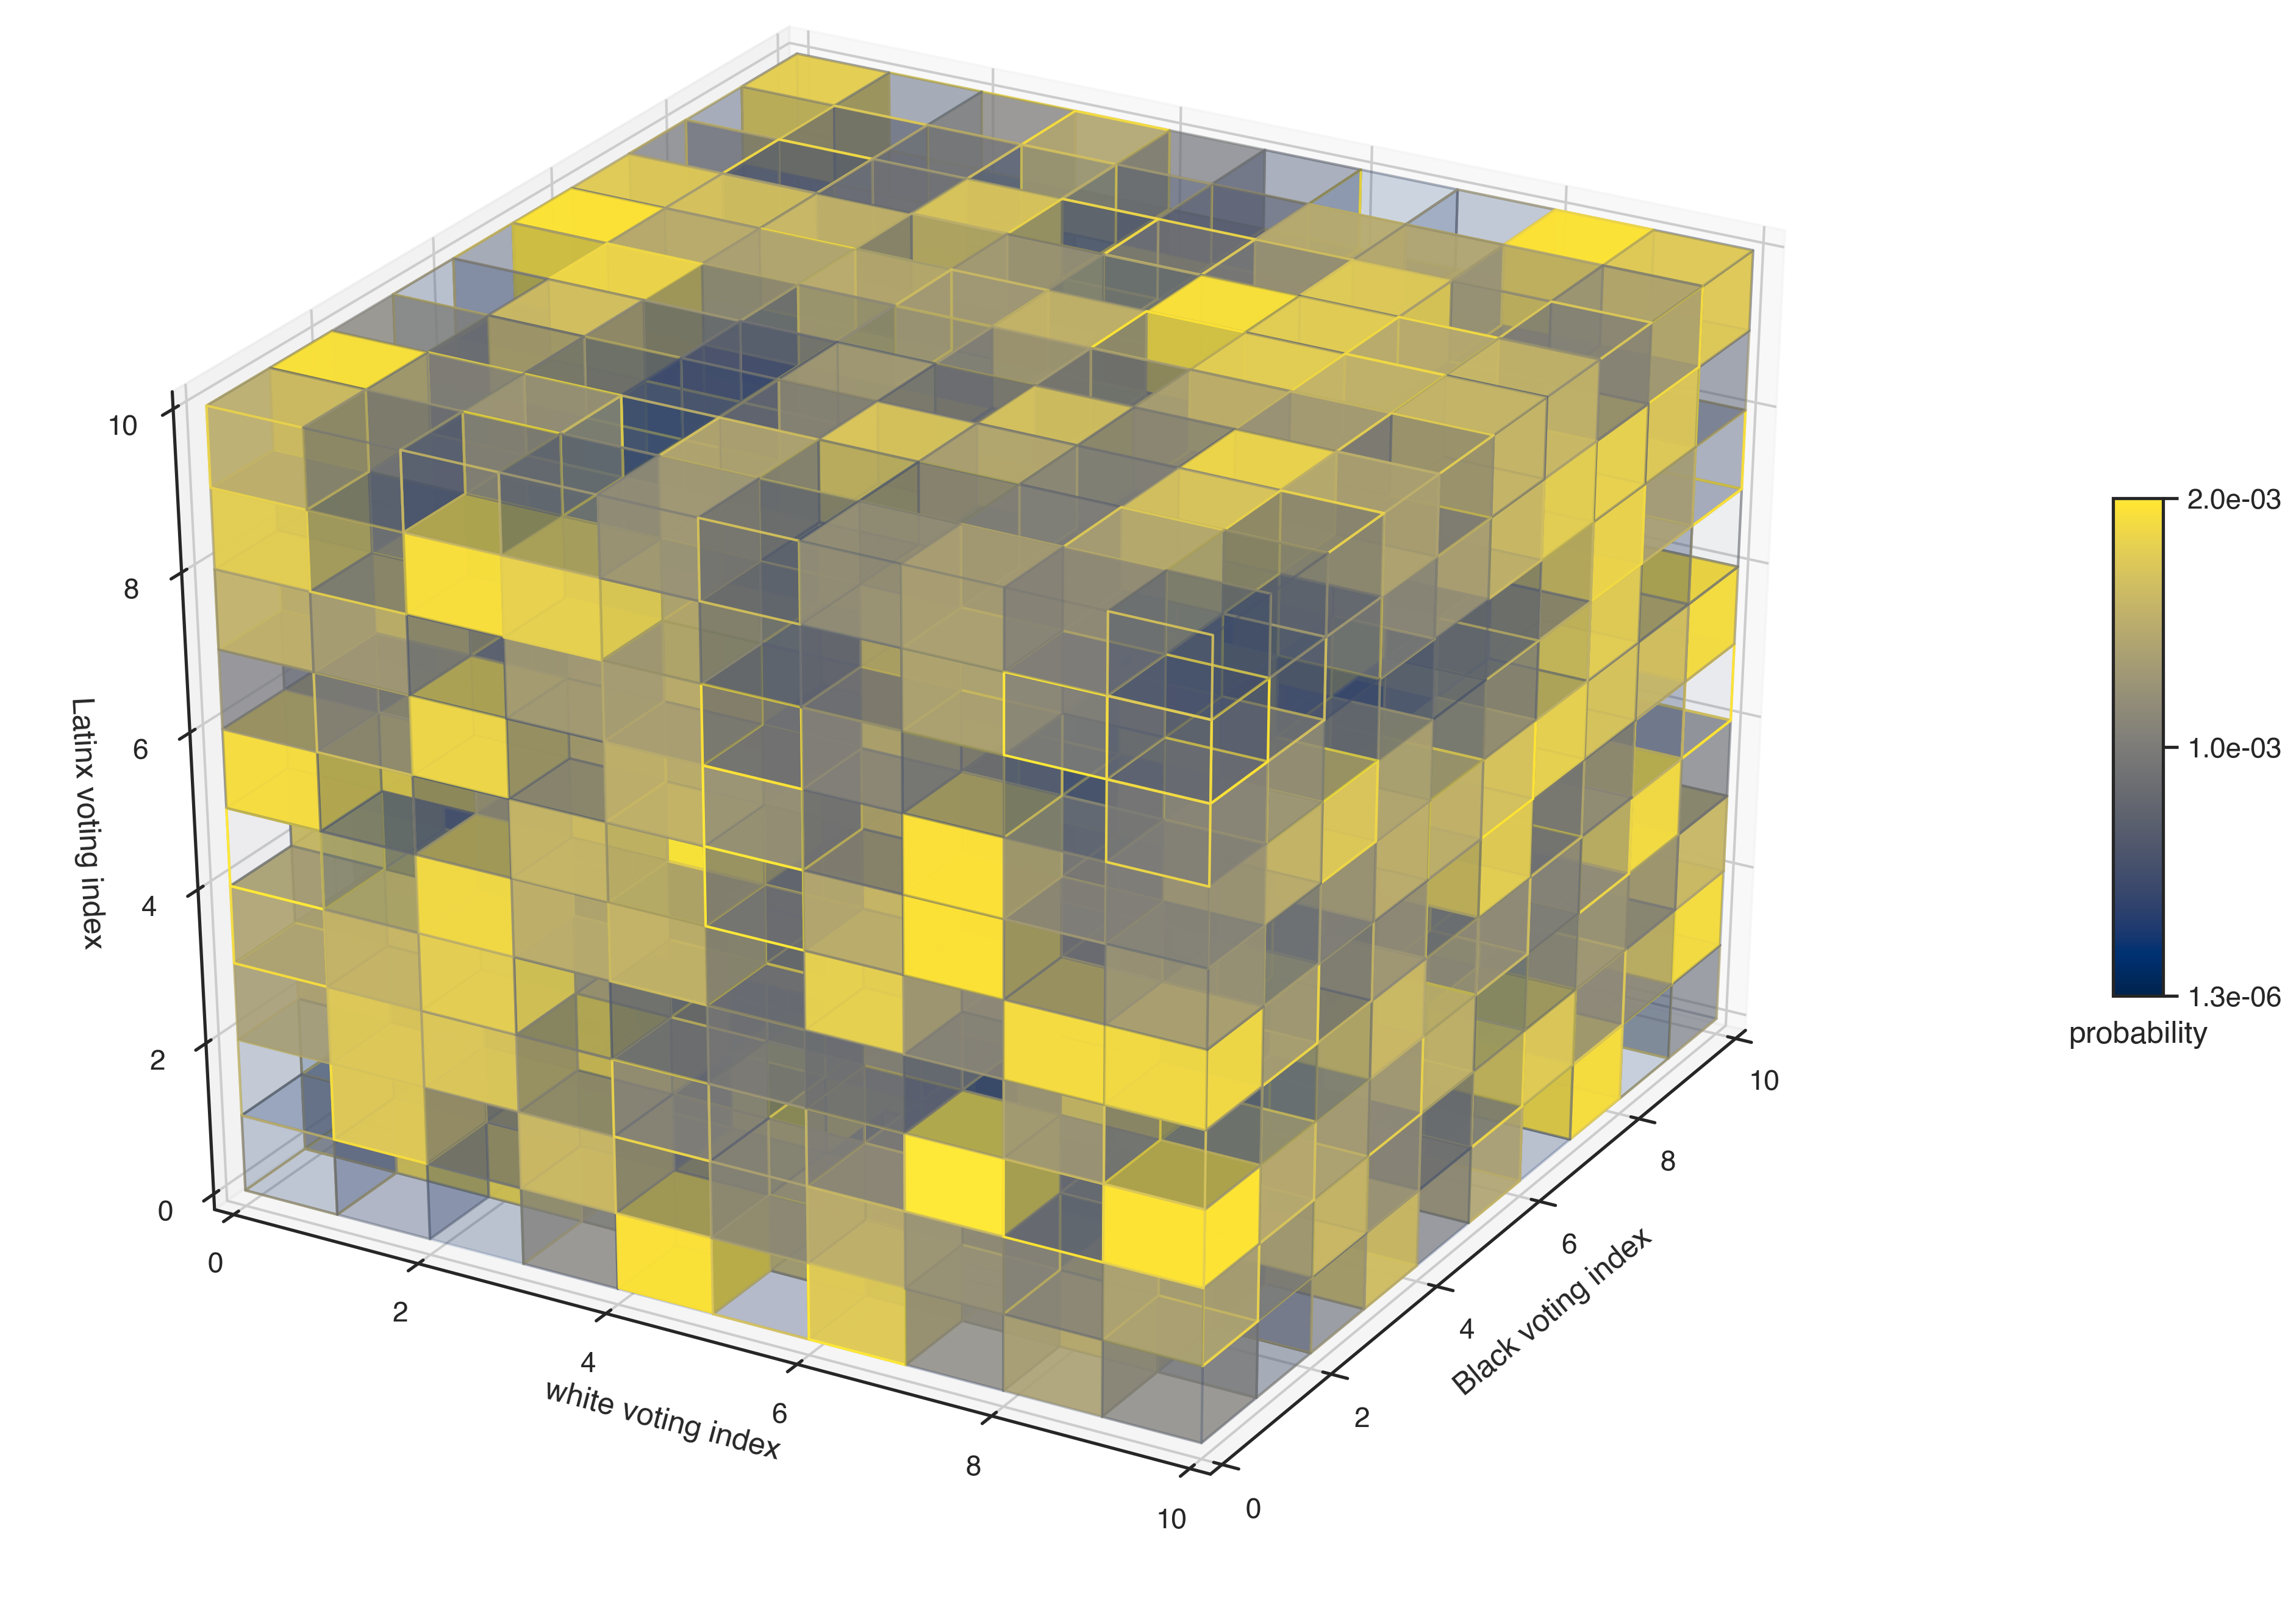
\includegraphics[width=\linewidth]{figures/3d_phc_plot_example.png}
 \caption{Example of a Rank $3$, Granularity $10$ Probabilistic Hypercube}
 \label{fig:3d_phc_plot_example}
\end{figure}

\begin{figure}[ht]\centering
 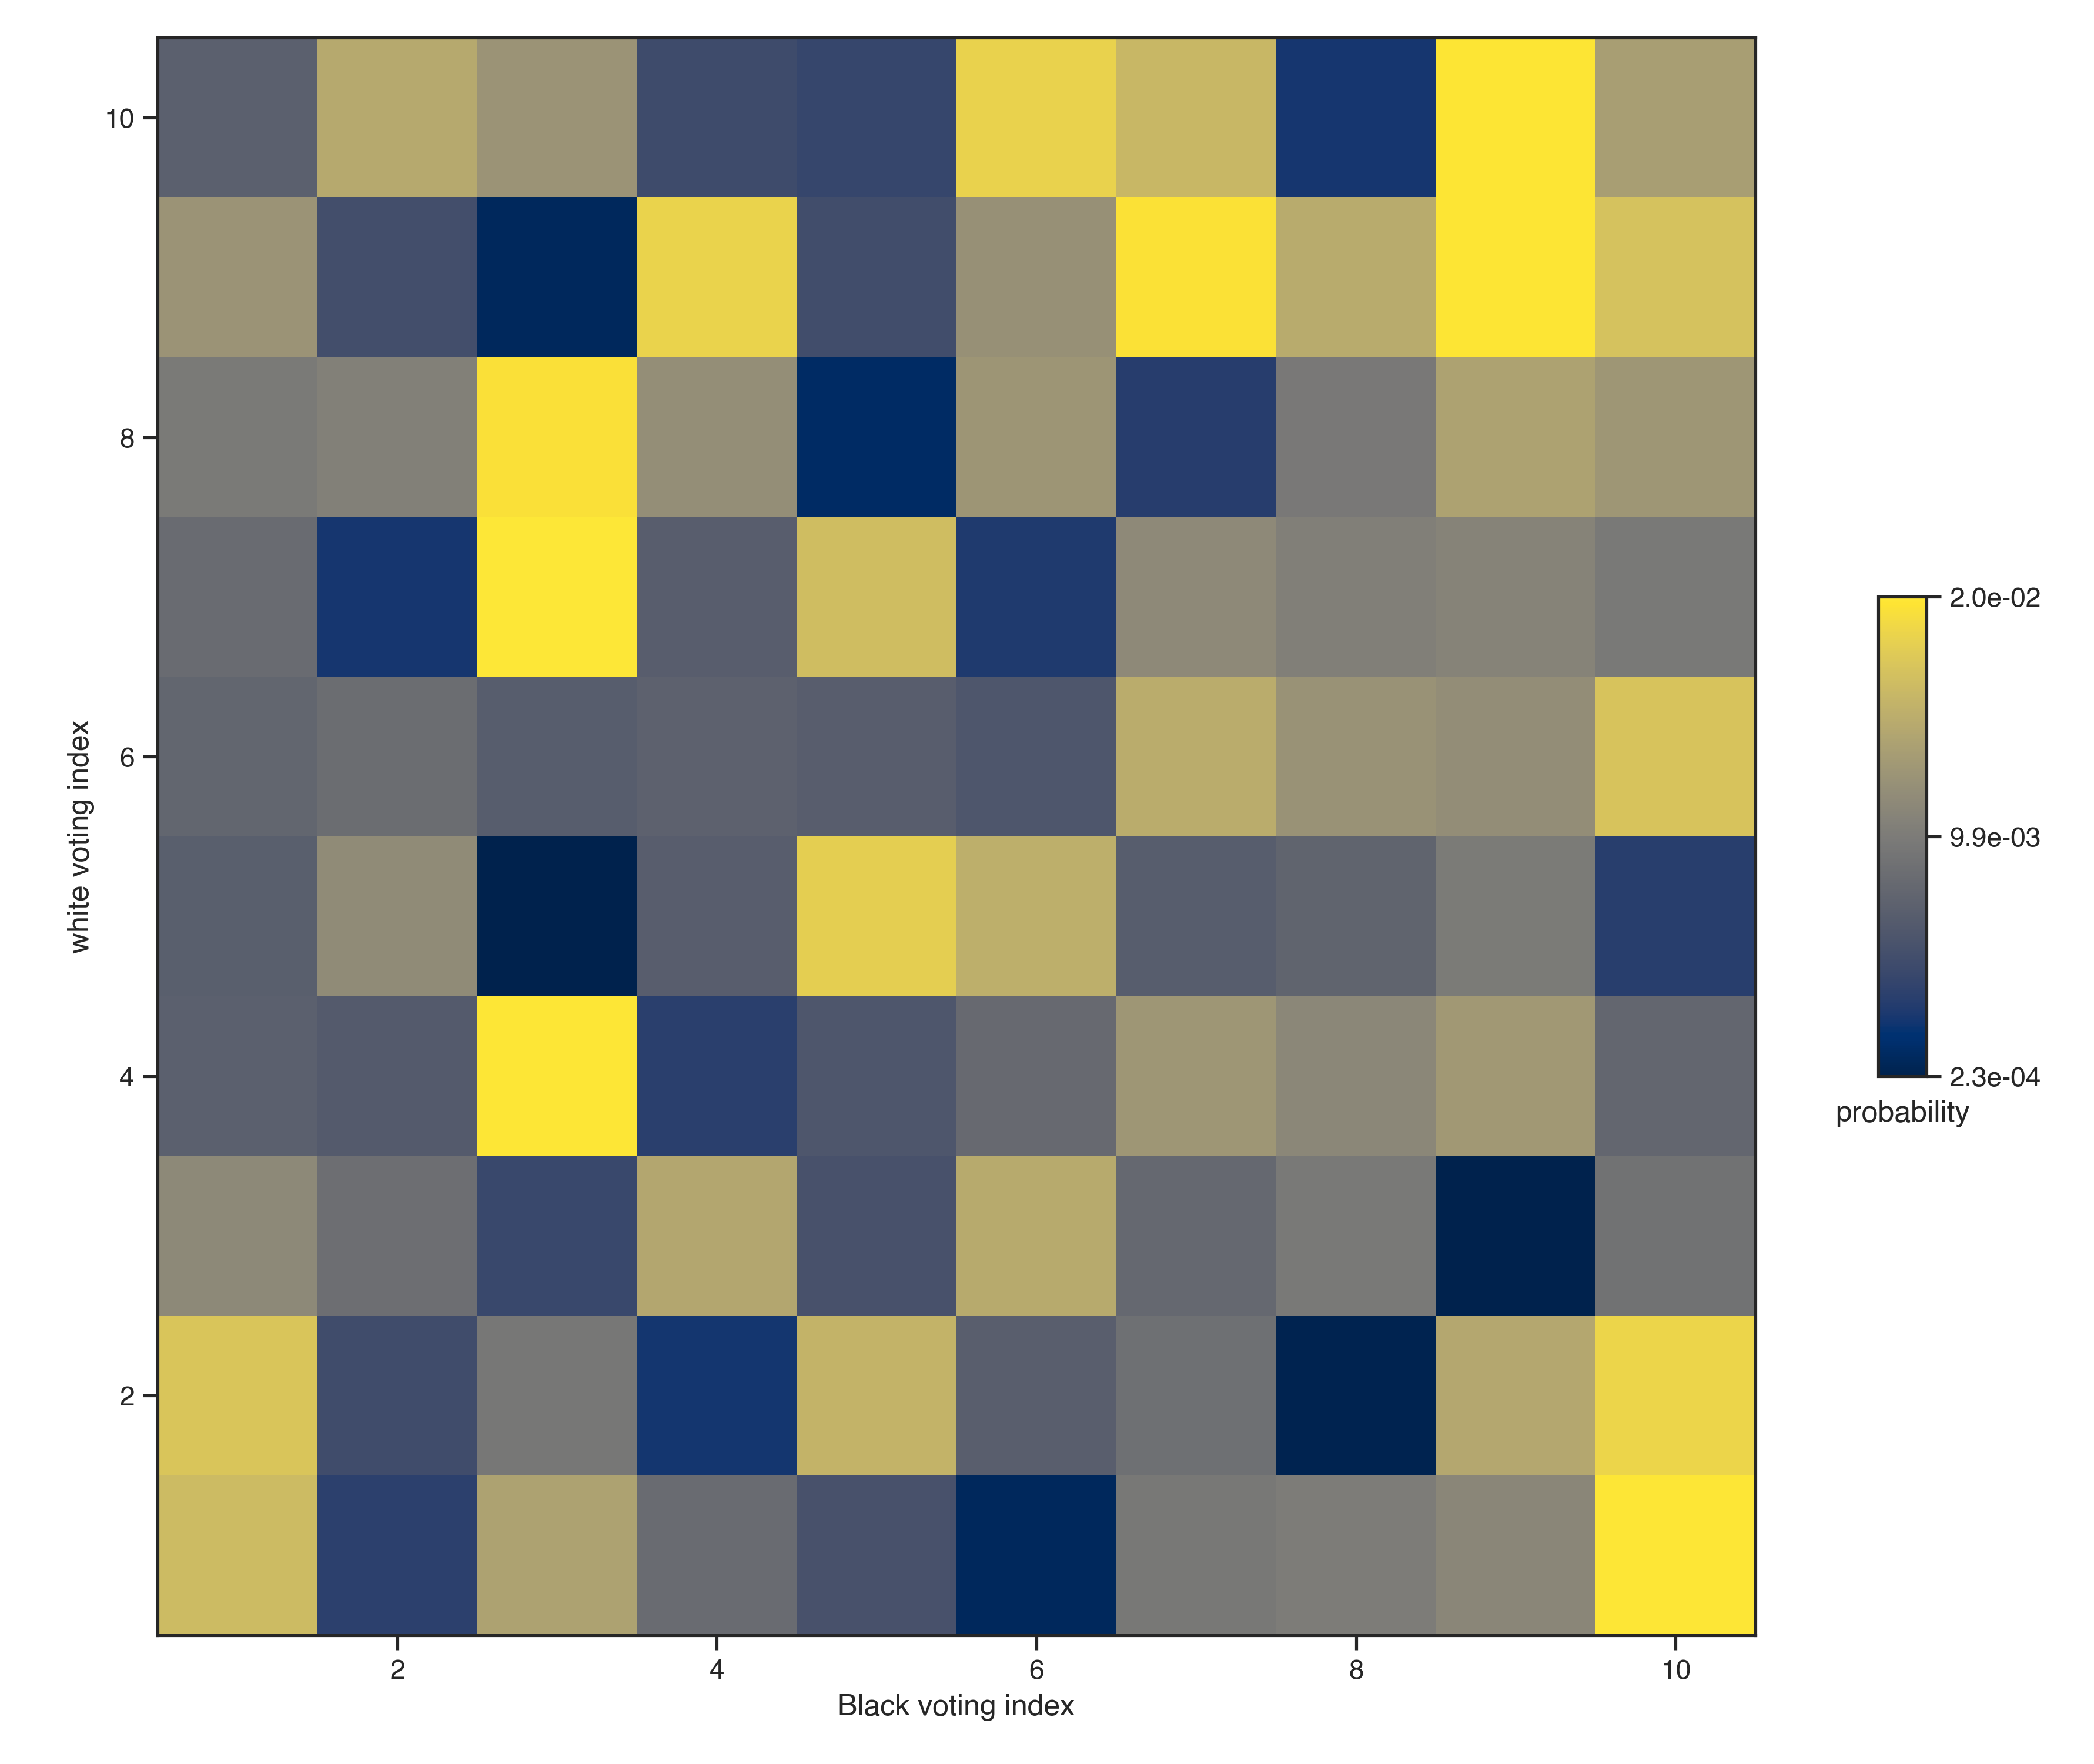
\includegraphics[width=\linewidth]{figures/2d_phc_plot_example.png}
 \caption{Example of a Rank $2$, Granularity $10$ Probabilistic Hypercube}
 \label{fig:2d_phc_plot_example}
\end{figure}

The rank $2$ case can also be visualized as a $3$-dimensional plot, where the third dimension is the probability associated with the cells of the PHC. Figure \ref{fig:2d_phc_plot_dist_example} illustrates this.

\begin{figure}[ht]\centering
 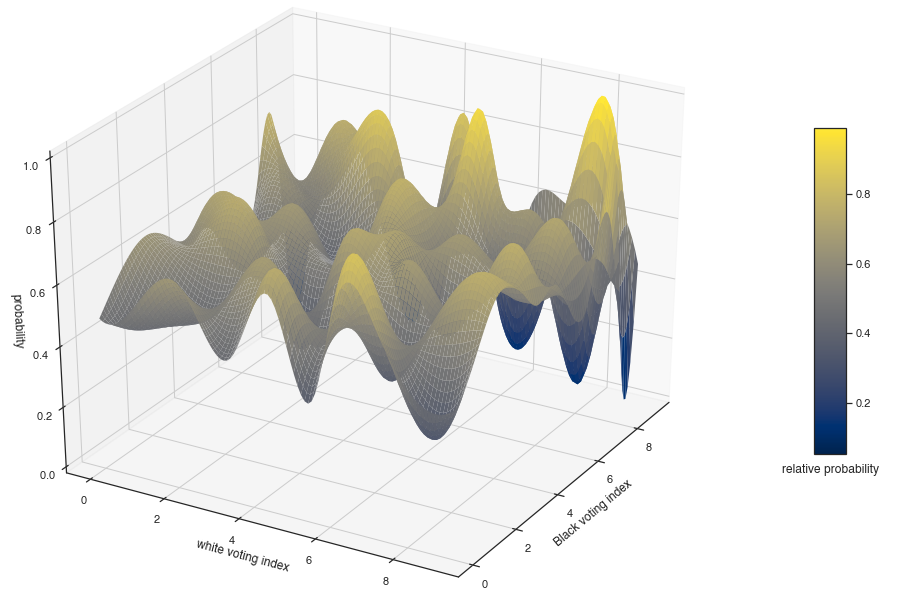
\includegraphics[width=\linewidth]{figures/2d_phc_plot_dist_example.png}
 \caption{The Probability Distribution within of a Rank $2$, Granularity $10$ Probabilistic Hypercube}
 \label{fig:2d_phc_plot_dist_example}
\end{figure}

Higher rank PHCs are difficult to visualize in similar ways, but the representational and intrinsic characteristics of the probability hypercube remain the same. This is critical to the Discrete Voter Model's ability to generalize to arbitrarily diverse electorates, with arbitrarily precise demographic voting probabilities.


\section{expec\_votes}

This is the first of two subroutines that score a candidate hypercube in every step of the Markov chain.

\texttt{expec\_votes} calculates the expectation of votes for a given candidate from some probabilistic hypercube.

The subroutine iterates over every cell in the hypercube and finds the expectation of votes that it dictates.

The notation is as follows:

\begin{itemize}
  \item $i = 0, 1, \dots, n$ represents cells in the hypercube
  \item $p_i$ represents the probability of being in cell $i$
  \item $j = 0, 1, \dots, r$ represents demographic groups
  \item $q_j$ represents the probability of demographic group $j$ to vote for the given candidate
  \item $m_j$ represents the population of demographic group $j$ in the district
\end{itemize}

The expectation of a hypercube is thus given by Equation \ref{eq:expec_votes}.

\begin{equation}
 \sum_{i = 0}^n p_i \left(\sum_{j = 0}^r q_j \cdot m_j\right)
 \label{eq:expec_votes}
\end{equation}

This expectation is then compared to the observed outcome of votes, with the $L1$-norm (absolute value). The lower the norm, the better the hypercube, and the more likely it will be accepted in the Markov chain.


\section{prob\_votes}

The is the second of two subroutines that score a candidate hypercube in every step of the Markov chain.

\texttt{prob\_votes} calculates the probability that a given hypercube produced the observed election outcome.

With the same notation as \texttt{expec\_votes}, and additionally:

\begin{itemize}
  \item $a_j$ represents the number of people in demographic group $j$ that voted for a candidate
  \item $d$ represents the observed number of votes cast for the given candidate
\end{itemize}

\begin{equation}
 \sum_{\forall a_j \text{ s.t. } \sum_{\forall j \in [0, r]} a_j = d} \left(\prod_{j = 0}^r q_j^{a_j} \cdot (1 - q_j)^{m_j - a_j}\right) \cdot \frac{d!}{\prod_{a_j}a_j!}
 \label{eq:prob_votes}
\end{equation}

In essence, Equation \ref{eq:prob_votes} uses the Binomial distribution to calculate the probability of members of different demographic groups voting together in a way to produce the desired outcome. This is extensible to any number of demographic groups and can be repeated for any number of candidates.

A crucial step in this process is generating all possible partitions of the observed electoral outcome into the demographic groups. For example, if $10$ people voted for a candidate, if there are three demographic groups, possible partitions include:

\begin{itemize}
  \item $4$ people from group $1$, $3$ people from group $2$, and $3$ people from group $3$ voted for the candidate
  \item $2$ people from group $1$, $0$ people from group $2$, and $8$ people from group $3$ voted for the candidate
  \item $4$ people from group $1$, $4$ people from group $2$, and $2$ people from group $3$ voted for the candidate
\end{itemize}

The code for this partitioning process can be found in the appendix, as Listing \ref{lst:integer_partition}.

The probability of some candidate hypercube producing the electoral outcome given by that expression is then compared to the probability that the current hypercube produced the outcome, and the candidate is accepted if the probability is higher, or with some acceptance probability if lower.

\section{elect}


\section{dvm}

The final subroutine, \texttt{mcmc}, runs the Markov chain Monte Carlo method with the Metropolis-Hastings algorithm, employing either \texttt{expec\_votes} or \texttt{prob\_votes} to score candidates.

The algorithm is as follows:

\begin{enumerate}
  \item initialize some hypercube with \texttt{make\_grid}
  \item iterate some number of times. at each iteration:
  \begin{enumerate}
    \item generate a candidate hypercube \\ with \texttt{shift\_weight}
    \item score that candidate with \\ \texttt{expec\_votes} or \texttt{prob\_votes}
    \item accept (assign it as the current hypercube and record the score) or reject that candidate based on the scores in the previous step
    \item if the score is better than all scores seen up until this point, save the score and the hypercube
  \end{enumerate}
  \item output all hypercubes explored, and identify the best scoring one
\end{enumerate}

The subroutine returns a collection of the best scoring hypercube, the highest score it received, and a list of all the hypercubes explored and their scores.


\texttt{shift\_weight}


The \texttt{shift\_weight} subroutine implements the proposal step of the MCMC method. It reversibly shifts the weight of the hypercube to create another hypercube. \textit{Reversibility} refers to an assumption of MCMC that guarantees convergence. A Markov chain is said to be reversible if there is a probability distribution, $\pi$, over the states such that:

$$\pi_i \text{Pr}(X_{n+1} = j | X_n = i) = \pi_j \text{Pr}(X_{n+1} = i | X_n = j)$$

for all iterations $n$ and all states $i$ and $j$. This is also called the \textit{detailed balance} condition.

\texttt{shift\_weight} allows for $5$ types of shifting:

\begin{enumerate}
  \item \texttt{uniform}: add a uniform random hypercube to the hypercube
  \item \texttt{single\_uniform}: add a single uniform random variable to each cell in the hypercube
  \item \texttt{shuffle}: shuffle the hypercube randomly
  \item \texttt{right}: shift weight in the hypercube to the right
  \item \texttt{left}: shift weight in the hypercube to the left
\end{enumerate}

Each of the above types of shifting is reversible, with the \texttt{uniform} as the default method. At each step of the chain, the algorithm uses this subroutine to propose a new hypercube.


\section{Evaluation}

All of the methods for inferring racially polarized voting noted above, including ecological regression, homoegenous precincts, and King's EI, are necessarily imperfect -- as is the Discrete Voter Model. The extent of that imperfection, however, can be evaluated and compared.

King's EI and the Discrete Voter Model are evaluated in this paper in two ways: accuracy and runtime. Both models are run on generated election data with different demographic distributions. The evaluation is only possible because with this generated election data, the ground truth, that is: the true demographic voting patterns, is known. That ground truth is fixed as an input in the \texttt{generate\_random\_election} subroutine, whose Python implementation can be found in Listing \ref{lst:election}.

The accuracy of the model is determined by how close the model's result is to the ground truth. The runtime of the model is how long it took the model to reach that result. Both are critically important to the model's use in practice.

DVM's runtime and accuracy are scored in comparison to King's EI for $2 \times 2$ examples, and demonstrations of its use on $R \times C$ examples are given in the \hyperref[sec:results]{Results} section.
